\documentclass[12pt,ngerman,a4paper,xcolor={dvipsnames}]{beamer}

\setlength{\parindent}{0pt}

\usepackage{babel}

\usepackage[utf8]{inputenc}
\usepackage[T1]{fontenc}
\usepackage{lmodern}



\usepackage{amsmath, amssymb,amsfonts,amsthm}


\usepackage{graphicx}


\usepackage{float}
\usepackage{listings}

\usepackage{hyperref}
\hypersetup{
	colorlinks=true,
	linkcolor=white,
	filecolor=magenta,      
	urlcolor=Salmon,}


\title{Projekt: Binäre Klassifikation}
\author{Nicolai Ülger, Niklas Mäschke, Suri Volz}
\date{Computerpraktikum, Juli 2020}
\usetheme{Berlin}
\usecolortheme{default}
\setbeamercolor{frametitle}{fg=white,bg=Salmon}
\setbeamercolor{title}{fg=white,bg=Salmon}
\setbeamercolor{section}{fg=white,bg=Salmon}
\setbeamertemplate{caption}[numbered]

\lstset{language=Python}

\newcommand{\hs}{\vspace{0.1cm}}
\begin{document}
\maketitle
\section{Aufgabenstellung}
\begin{frame}{Aufgaben}
	\begin{itemize}
		\item Implementierung eines Verfahrens zur binären Klassifikation
		\item Visualisierung für zweidimensionale Datensätze
		\item Einfügen eines Kommandozeilen-Interface 
	\end{itemize}
	
\end{frame}

\section{Verfahren}


\begin{frame}{K-nearest-Neighbours}
	Bestimmung der k nächsten Nachbarn eines Punktes über kd Trees
	\begin{figure}[h]
		\centering
		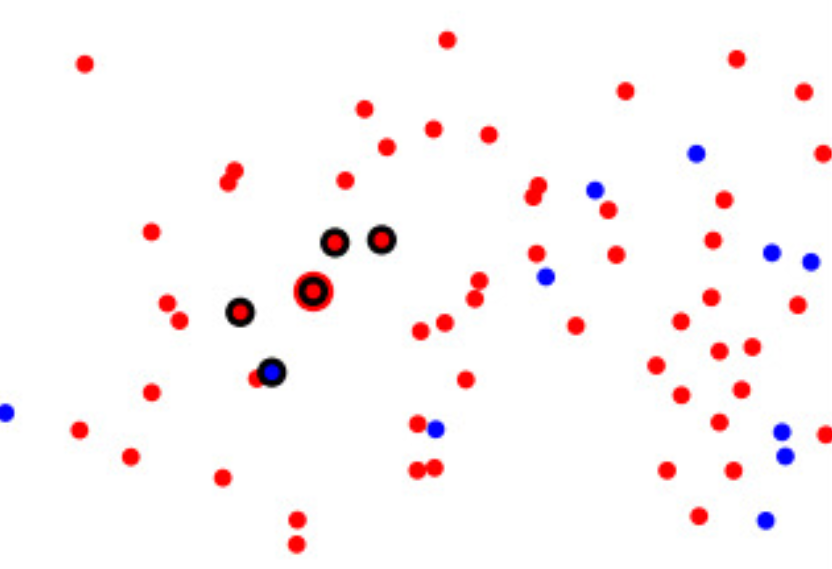
\includegraphics[width=6cm, height=4cm]{knn}
		\caption{knN, wobei k=4}
	\end{figure}

\end{frame}
\begin{frame}{$f_{D,k}$}
	Klassifikation eines Punktes über  $f_{D,k}=sign(\sum_{j=1}^{k}y_{i_{j} })$, wobei $sign(0):=1$. 
	
	
	
	
\end{frame}
\begin{frame}{Fehlerklassifikationsrate $R$}
		Danach wird die Fehlklassifikationsrate $R_{Di}(f_{D\backslash i,k})$  für jede Teilmenge bestimmt und der Mittelwert gebildet. Der kleinste Mittelwert gibt $k*$.
\end{frame}

\begin{frame}{Ergebnis}
	Dieses $f_{D,k*}$ wird auf die Trainingsdatei angewandt, wobei zusätzlich die Klassifikationsfehelerrate ausgegeben wird.	
\end{frame}

\begin{frame}{Live Demonstration}
	Live Demonstration 
\end{frame}

\begin{frame}{Helper Methods}
	\begin{itemize}
		\item Die csv-Datei wird ausgelesen und in l Teilmengen gesplittet
		\item Die Ergebnisse werden geplottet
	\end{itemize}
	
\end{frame}


\section{Code}

\begin{frame}{GitHub}
	Code zum downloaden auf Github: \url{https://github.com/uelgerni/KI-Projekt}
\end{frame}
\end{document}	